\documentclass[miniframe]{lbpbeamer}
%\documentclass[handout]{lbpbeamer}
%%%%%%%%%%%%% option de la classe lbpbeamer.cls
% toutes les options standards de la classe beamer
% le type d'en-tete pour l'appel des sections : 
%  - default : currentsection | currentsubsection
%  - miniframe : sections + puces
%  - tree : sections + currentsubsection
%  - split : sections + subsections
%%%%%%%%%%%%%%%%%%%%%%%%%%%%%%%%%%%%%%%%%%%%%%%%%%

%%%%%%%%%%%%% appel des packages
\usepackage[english,french]{babel}
\usepackage{epsfig}
\usepackage[T1]{fontenc}
\usepackage[utf8]{inputenc}
\usepackage{lmodern} 
\usepackage{times}
\usepackage{multirow}
\usepackage{animate}
\usepackage{hyperref}
\usepackage{movie15}
\usepackage{wasysym}
\usepackage[squaren, Gray, cdot]{SIunits}
\usepackage{tikz}
\usetikzlibrary{calc,trees,positioning,arrows,arrows.meta,chains,shapes.geometric,%
	decorations.pathreplacing,decorations.pathmorphing,shapes,%
matrix,shapes.symbols,plotmarks,decorations.markings,shadows}

\usepackage{tabularx}
\newcolumntype{L}[1]{>{\raggedright\let\newline\\\arraybackslash\hspace{0pt}}m{#1}}
\newcolumntype{C}[1]{>{\centering\let\newline\\\arraybackslash\hspace{0pt}}m{#1}}
\newcolumntype{R}[1]{>{\raggedleft\let\newline\\\arraybackslash\hspace{0pt}}m{#1}}

\newcommand{\backupbegin}{
	\newcounter{framenumberappendix}
	\setcounter{framenumberappendix}{\value{framenumber}}
}
\newcommand{\backupend}{
	\addtocounter{framenumberappendix}{-\value{framenumber}}
	\addtocounter{framenumber}{\value{framenumberappendix}} 
}

%\usepackage{enumitem}

%%%%%%%%%%%%%%%%%%%%%%%%%%%%%%%%%%%%%%%%%%%%%%%%%%
%\newlist{fleche}{itemize}{1}
%\setlist[fleche]{label=$\rightarrow$,font=\color{blue}}


%\newcommand{\smiley}{\tikz[baseline=-0.75ex,black]{
%		    \draw circle (2mm);
%			\node[fill,circle,inner sep=0.5pt] (left eye) at (135:0.8mm) {};
%			\node[fill,circle,inner sep=0.5pt] (right eye) at (45:0.8mm) {};
%			\draw (-145:0.9mm) arc (-120:-60:1.5mm);
%			    }
%			}

\newcommand{\orto}{^{\circ}}

%%%%%%%%%%%%% appel du plan a chaque subsection
%% en 1 colonne

%\AtBeginSection[]{
%	\frame{%<handout:0>{
%	\frametitle{Plan}
%  \begin{columns}[t]
%  \begin{column}{0.5\linewidth}
%  \tableofcontents[sections={1-3}, currentsection,subsectionstyle=show/show/shaded]
%  \end{column}
%  \begin{column}{0.5\linewidth}
%  \tableofcontents[sections={4-6}, currentsection,subsectionstyle=show/show/shaded]
%  \end{column}
%  \end{columns}
%  }
%}

%% ou en 2 colonnes s'il y a trop de sections
    
%\AtBeginSubsection[]{
%	\frame{%<handout:0>{
%	\frametitle{Summary}
%  \begin{columns}[t]
%  \begin{column}{0.5\linewidth}
%  \tableofcontents[sections={1-6},currentsection, subsectionstyle=show/shaded/hide]
%  \end{column}
%  \begin{column}{0.5\linewidth}
%  \tableofcontents[sections={7-12},currentsection,subsectionstyle=show/shaded/hide]
%  \end{column}
%  \end{columns}
%  }
%}	
%%%%%%%%%%%%%%%%%%%%%%%%%%%%%%%%%%%%%%%%%%%%%%%%%%	

%%%%%%%%%%%%% Pour supprimer les symboles de navigation
\setbeamertemplate{navigation symbols}{}
%%%%%%%%%%%%%%%%%%%%%%%%%%%%%%%%%%%%%%%%%%%%%%%%%%

%%%%%%%%%%%%% Personnalisation des theoremes
\newtheorem{theoreme}{Th\'eor\`eme}
\newtheorem{preuve}{D\'emonstration}
\newtheorem{define}{D\'efinition}
%%%%%%%%%%%%%%%%%%%%%%%%%%%%%%%%%%%%%%%%%%%%%%%%%%	
		
%%%%%%%%%%%%% Infos personnelles au document	
\title[Introduction à SysML]{Introduction à SysML}
\subtitle{Langage de modélisation graphique de systèmes}
\author[Fiack]{Laurent Fiack}
%\email{}
\institute[Lycée Blaise Pascal]{Lycée Blaise Pascal}
\date[\today]{\today}
\logo{
\includegraphics[scale=0.3]{./figures/logo_sysml.png}\hspace{1em}}
%%%%%%%%%%%%%%%%%%%%%%%%%%%%%%%%%%%%%%%%%%%%%%%%%%

\newcommand{\figpath}{figures/}

\usepackage{scrextend}

\begin{document}

%%%%%%%%%%%%% Background des slides	
\usebackgroundtemplate{}
%% cet option permet d'ins\'erer une image en fond-ecran
%% la commande \usebackgroundtemplate{} permet de
%% supprimer le fond a partir du moment ou il est 
%% appele
%%%%%%%%%%%%%%%%%%%%%%%%%%%%%%%%%%%%%%%%%%%%%%%%%%	

%%%%%%%%%%%%% frame title
\frame{\titlepage}
\usebackgroundtemplate{}
\logo{}
%\logoheader{taille}{emplacement-image}
%% on supprime les logos des autres frames		
%%%%%%%%%%%%%%%%%%%%%%%%%%%%%%%%%%%%%%%%%%%%%%%%%%
\section[SysML ?]{SysML ?}
\subsection[SysLM]{SysML}
%\frame{
%	\frametitle{SysML ?}
%	\small
%	\begin{minipage}[b]{0.58\linewidth}
%		\begin{block}{Définition d'un système}
%			Un système est un ensemble de constituant inter-reliés qui interagissent les uns avec les autres d'une manière organisée pour accomplir une finalité commune.
%		\end{block}
%	\end{minipage}
%	\hfill
%	\begin{minipage}[b]{0.38\linewidth}
%		\centering
%		
\includegraphics[scale=.3]{./figures/logo_sysml.png}
%	\end{minipage}
%
%	\vspace{3em}
%
%	\begin{addmargin}[2em]{2em}
%		SysML est un \textbf{langage de modélisation graphique} dérivé d'UML.\\
%		Ce langage va bien au delà des problématiques de l'informatique.\\ 
%		Comme UML, \textbf{SysML n’est pas une méthode}.\\
%	\end{addmargin}
%}

\frame{
	\frametitle{SysML}
	\footnotesize
	\begin{block}{Pourquoi a-t-on besoin d'un langage de modélisation ?}
		\begin{itemize}
			\item Les systèmes sont devenus plus complexes et pluritechniques, un besoin de langage transversal et unifié apparait.
			\item Il doit permettre à des acteurs de corps de métiers différents de collaborer autour d’un modèle commun pour définir un système.
			\item On favorise la création de bibliothèques de systèmes, ainsi que la réutilisation de librairie de systèmes, permettant un gain de productivité.
		\end{itemize}
	\end{block}
	\begin{block}{Qui utilise SysML ?}
		\centering
		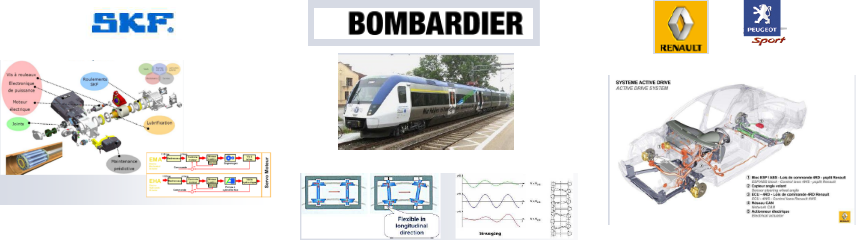
\includegraphics[scale=.4]{./figures/boites_sysml.png}
	\end{block}
}

\frame{
	\frametitle{Qui utilise SysML ?}
	\tiny
	\begin{minipage}[t]{0.48\linewidth}
		\begin{itemize}
			\item "Blohm + Voss Naval GmbH" - bateaux, logistique
			\item "VEGA Space GmbH",- aérospace
			\item "MIT Lincoln Laboratory" - Institute Technologie de Massachusetts
			\item "Lockheed Martin MS2" – militaire
			\item "Lockheed Martin" – militaire
			\item "US Army" – militaire
			\item "ESO - European Organisation for Astronomical Research" – aerospace
			\item "Boeing"
			\item "Raytheon"
			\item "CNES" – France
			\item "Thales" – France
			\item "ESA" - European Space Agency
			\item "NASA"
		\end{itemize}
	\end{minipage}
	\hfill
	\begin{minipage}[t]{0.48\linewidth}
		\begin{itemize}
			\item "BMW"
			\item "Sopra Group" – France
			\item "Thales Security Solutions and Services" – France
			\item "Rockwell Collins Inc."
			\item "JPL" – coentreprise avec la NASA
			\item "GE Aviation"
			\item "GE Transportation" - France, Italie
			\item "NEWTEC LLC"
			\item "NASA Langley Research Center"
			\item "BAE Systems", - France
			\item "Siemens AG"
			\item "Philips"
			\item "NASA Goddard Space Flight Center"
			\item "Bombardier Transportation GmbH"
			\item "Bombardier Transportation Italy"
		\end{itemize}
	\end{minipage}

	\vspace{1em}
	\small ...et bien d'autres !
}

\definecolor{lorange}{RGB}{250,214,185}
\definecolor{lyellow}{RGB}{250,250,100}
\definecolor{lred}{RGB}{230,156,164}
\frame{
	\frametitle{SysML, l'ensemble des 9 diagrammes}
	\begin{center}
		\footnotesize
		\begin{block}{Définition d'un système}
			Un système est un ensemble de constituant inter-reliés qui interagissent les uns avec les autres d'une manière organisée pour accomplir une finalité commune.
		\end{block}
		\vspace{1em}
		\tiny
		\begin{tikzpicture}[scale=.6]
			\draw[drop shadow, fill=lorange] (-2.5,-0.5) rectangle (2.5,0.5);
			\draw (0,0) node{Diagramme SysML};

			\draw[drop shadow, fill=lorange] (-7.5,-1.5) rectangle (-2.5,-2.5);
			\draw (-5,-2) node{Diagramme comportemental};

			\draw[drop shadow, fill=lorange] (7.5,-1.5) rectangle (2.5,-2.5);
			\draw (5,-2) node{Diagramme structurel};

			\draw[drop shadow, fill=lyellow] (-1.5,-1.5) rectangle (1.5,-2.5);
			\draw (0,-2) node[align=center]{Diagramme \\ d'exigences};

			\draw[drop shadow, fill=lyellow] (-9.5,-3.5) rectangle (-6.5,-4.5);
			\draw (-8,-4) node[align=center]{Diagramme \\ d'activité};

			\draw[drop shadow, fill=lyellow] (-5.5,-3.5) rectangle (-2.5,-4.5);
			\draw (-4,-4) node[align=center]{Diagramme \\ d'états};

			\draw[drop shadow, fill=lyellow] (-0.5,-3.5) rectangle (2.5,-4.5);
			\draw (1,-4) node[align=center]{Diagramme de \\ définition de block};

			\draw[drop shadow, fill=lyellow] (3.5,-3.5) rectangle (6.5,-4.5);
			\draw (5,-4) node[align=center]{Diagramme de \\ bloc interne};

			\draw[drop shadow, fill=lyellow] (7.5,-3.5) rectangle (10.5,-4.5);
			\draw (9,-4) node[align=center]{Diagramme de \\ packages};

			\draw[drop shadow, fill=lyellow] (-8.5,-5.5) rectangle (-5.5,-6.5);
			\draw (-7,-6) node[align=center]{Diagramme de \\ séquence};

			\draw[drop shadow, fill=lyellow] (-5,-5.5) rectangle (-1,-6.5);
			\draw (-3,-6) node[align=center]{Diagramme de cas \\ d'utilisation};

			\draw[drop shadow, fill=lyellow] (3.5,-5.5) rectangle (6.5,-6.5);
			\draw (5,-6) node[align=center]{Diagramme \\ paramétrique};

			\draw (-5,-1.5) -- (-5,-1) -- (5,-1) -- (5,-1.5);
			\draw[->] (0,-1.5) -- (0,-0.5);

			\draw (-8,-3) -- (-2,-3);
			\draw (-8,-3.5) -- (-8,-3);
			\draw (-4,-3.5) -- (-4,-3);
			\draw (-6,-5.5) -- (-6,-3);
			\draw (-2,-5.5) -- (-2,-3);
			\draw[->] (-5,-3) -- (-5,-2.5);

			\draw (1,-3.5) -- (1,-3) -- (9,-3) -- (9,-3.5);
			\draw[->] (5,-3.5) -- (5,-2.5);
			
			\draw[->] (5,-5.5) -- (5,-4.5);

		\end{tikzpicture}

\end{center}
}

\frame{
	\frametitle{STI2D : Les six diagrammes au programme}
	\begin{center}
		\tiny
		\begin{tikzpicture}[scale=.6]
			\draw[drop shadow, fill=lorange] (-2.5,-0.5) rectangle (2.5,0.5);
			\draw (0,0) node{Diagramme SysML};

			\draw[drop shadow, fill=lorange] (-7.5,-1.5) rectangle (-2.5,-2.5);
			\draw (-5,-2) node{Diagramme comportemental};

			\draw[drop shadow, fill=lorange] (7.5,-1.5) rectangle (2.5,-2.5);
			\draw (5,-2) node{Diagramme structurel};

			\draw[drop shadow, fill=lyellow] (-1.5,-1.5) rectangle (1.5,-2.5);
			\draw (0,-2) node[align=center]{Diagramme \\ d'exigences};

			\draw[drop shadow, fill=gray] (-9.5,-3.5) rectangle (-6.5,-4.5);
			\draw (-8,-4) node[align=center]{Diagramme \\ d'activité};

			\draw[drop shadow, fill=lyellow] (-5.5,-3.5) rectangle (-2.5,-4.5);
			\draw (-4,-4) node[align=center]{Diagramme \\ d'états};

			\draw[drop shadow, fill=lyellow] (-0.5,-3.5) rectangle (2.5,-4.5);
			\draw (1,-4) node[align=center]{Diagramme de \\ définition de block};

			\draw[drop shadow, fill=lyellow] (3.5,-3.5) rectangle (6.5,-4.5);
			\draw (5,-4) node[align=center]{Diagramme de \\ bloc interne};

			\draw[drop shadow, fill=gray] (7.5,-3.5) rectangle (10.5,-4.5);
			\draw (9,-4) node[align=center]{Diagramme de \\ packages};

			\draw[drop shadow, fill=lyellow] (-8.5,-5.5) rectangle (-5.5,-6.5);
			\draw (-7,-6) node[align=center]{Diagramme de \\ séquence};

			\draw[drop shadow, fill=lyellow] (-5,-5.5) rectangle (-1,-6.5);
			\draw (-3,-6) node[align=center]{Diagramme de cas \\ d'utilisation};

			\draw[drop shadow, fill=gray] (3.5,-5.5) rectangle (6.5,-6.5);
			\draw (5,-6) node[align=center]{Diagramme \\ paramétrique};

			\draw (-5,-1.5) -- (-5,-1) -- (5,-1) -- (5,-1.5);
			\draw[->] (0,-1.5) -- (0,-0.5);

			\draw (-8,-3) -- (-2,-3);
			\draw (-8,-3.5) -- (-8,-3);
			\draw (-4,-3.5) -- (-4,-3);
			\draw (-6,-5.5) -- (-6,-3);
			\draw (-2,-5.5) -- (-2,-3);
			\draw[->] (-5,-3) -- (-5,-2.5);

			\draw (1,-3.5) -- (1,-3) -- (9,-3) -- (9,-3.5);
			\draw[->] (5,-3.5) -- (5,-2.5);
			
			\draw[->] (5,-5.5) -- (5,-4.5);

		\end{tikzpicture}
	\end{center}
}

\frame{
	\frametitle{Application du langage SysML sur un exemple}
	\begin{minipage}[b]{0.38\linewidth}
		\footnotesize
		\begin{block}{Spot motorisé}
			\begin{itemize}
				\item Il doit permettre à distance la commande de l’orientation de la lumière afin de pouvoir éclairer une zone particulière d’un tableau de maître.
				\item La demande émane de galeristes d’Honfleur, qui doivent souvent réorienter leur éclairage en fonction des tableaux exposés dans leurs galeries.
			\end{itemize}
		\end{block}
		\vspace{2em}
	\end{minipage}
	\hfill
	\begin{minipage}[b]{0.58\linewidth}
		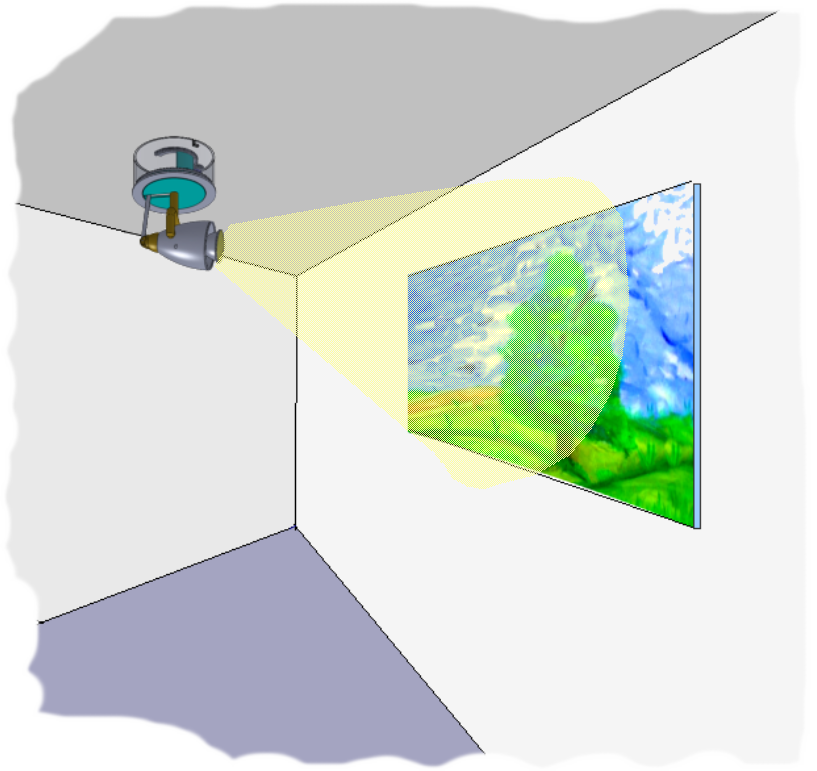
\includegraphics[width=\linewidth]{./figures/spot1.png}
	\end{minipage}
}

\frame{
	\frametitle{SysML, un langage de modélisation graphique}
	\vspace{-1em}
	\begin{center}
		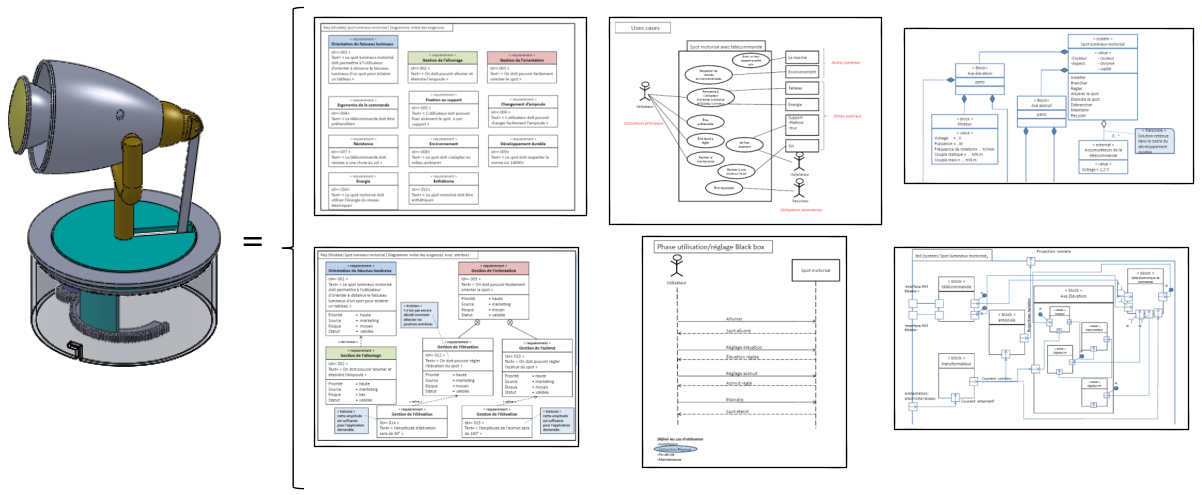
\includegraphics[width=.8\linewidth]{./figures/spot2.png}
	\end{center}
	\vspace{-1em}
	\footnotesize
	\begin{minipage}[b]{0.28\linewidth}
		Projet étudié,
	\end{minipage}
	\hfill
	\begin{minipage}[b]{0.68\linewidth}
		6 diagrammes permettent de décrire un produit.
	\end{minipage}
	\scriptsize
	\begin{block}{SysML est fait pour}
		\begin{itemize}
			\item Spécifier les systèmes.
			\item Analyser la structure et le fonctionnement des systèmes.
			\item Décrire les systèmes et concevoir des systèmes composés de sous systèmes.
			\item Vérifier et valider la faisabilité d'un système avant sa réalisation.
		\end{itemize}
	\end{block}
}

\frame{
	\frametitle{Diagramme de cas d'utilisation}
	\begin{center}
		\tiny
		\begin{tikzpicture}[scale=.6]
			\draw[drop shadow, fill=lorange] (-2.5,-0.5) rectangle (2.5,0.5);
			\draw (0,0) node{Diagramme SysML};

			\draw[drop shadow, fill=lorange] (-7.5,-1.5) rectangle (-2.5,-2.5);
			\draw (-5,-2) node{Diagramme comportemental};

			\draw[drop shadow, fill=lorange] (7.5,-1.5) rectangle (2.5,-2.5);
			\draw (5,-2) node{Diagramme structurel};

			\draw[drop shadow, fill=lyellow] (-1.5,-1.5) rectangle (1.5,-2.5);
			\draw (0,-2) node[align=center]{Diagramme \\ d'exigences};

			\draw[drop shadow, fill=gray] (-9.5,-3.5) rectangle (-6.5,-4.5);
			\draw (-8,-4) node[align=center]{Diagramme \\ d'activité};

			\draw[drop shadow, fill=lyellow] (-5.5,-3.5) rectangle (-2.5,-4.5);
			\draw (-4,-4) node[align=center]{Diagramme \\ d'états};

			\draw[drop shadow, fill=lyellow] (-0.5,-3.5) rectangle (2.5,-4.5);
			\draw (1,-4) node[align=center]{Diagramme de \\ définition de block};

			\draw[drop shadow, fill=lyellow] (3.5,-3.5) rectangle (6.5,-4.5);
			\draw (5,-4) node[align=center]{Diagramme de \\ bloc interne};

			\draw[drop shadow, fill=gray] (7.5,-3.5) rectangle (10.5,-4.5);
			\draw (9,-4) node[align=center]{Diagramme de \\ packages};

			\draw[drop shadow, fill=lyellow] (-8.5,-5.5) rectangle (-5.5,-6.5);
			\draw (-7,-6) node[align=center]{Diagramme de \\ séquence};

			\draw[drop shadow, fill=lyellow] (-5,-5.5) rectangle (-1,-6.5);
			\draw (-3,-6) node[align=center]{Diagramme de cas \\ d'utilisation};

			\draw[drop shadow, fill=gray] (3.5,-5.5) rectangle (6.5,-6.5);
			\draw (5,-6) node[align=center]{Diagramme \\ paramétrique};

			\draw (-5,-1.5) -- (-5,-1) -- (5,-1) -- (5,-1.5);
			\draw[->] (0,-1.5) -- (0,-0.5);

			\draw (-8,-3) -- (-2,-3);
			\draw (-8,-3.5) -- (-8,-3);
			\draw (-4,-3.5) -- (-4,-3);
			\draw (-6,-5.5) -- (-6,-3);
			\draw (-2,-5.5) -- (-2,-3);
			\draw[->] (-5,-3) -- (-5,-2.5);

			\draw (1,-3.5) -- (1,-3) -- (9,-3) -- (9,-3.5);
			\draw[->] (5,-3.5) -- (5,-2.5);
			
			\draw[->] (5,-5.5) -- (5,-4.5);

			\draw[ultra thick, red, rounded corners=3] (-5.2,-5.3) rectangle (-0.8,-6.7);
		\end{tikzpicture}
	\end{center}
}

\section[uc]{Diagramme de cas d'utilisation}
\subsection[uc]{Diagramme de cas d'utilisation}
\frame{
	\frametitle{Diagramme de cas d'utilisation}
	\begin{center}
		\textbf{En anglais :} \emph{Use case diagram}\\
		\textbf{Abrégé :} \texttt{uc}
		\small
		\begin{block}{Objectifs}
%			Ce diagramme permet de représenter les besoins attendus par un système.
			Recenser les besoins clients et délimiter précisément le système,
			en recherchant les \textbf{acteurs}, ceux qui ont des \textbf{interactions} avec lui, et les \textbf{cas d’utilisation}, ce à quoi sert le système.
		\end{block}
		\begin{block}{Définition}
			Le diagramme de cas d’utilisation est un schéma qui montre les \textbf{cas d’utilisation} (ovales) 
			reliés par des \textbf{associations} (lignes) à leurs \textbf{acteurs} (icône d'un stick man). 

			Chaque association signifie simplement \og{}participe à\fg{}.
		\end{block}
	\end{center}
}

\frame{
	\frametitle{UC : exemple du spot lumineux}
	\begin{center}
		\tiny
		\begin{tikzpicture}[scale=.6]
			\onslide<1->{
			\draw (0,0) rectangle (18,-12);
			\draw (0,0) node[below right]{\textbf{uc} [Modèle] Spot lumineux [Cas d'utilisation du spot lumineux]};
			}

			\onslide<2->{
			\draw (4,-1) rectangle (14,-11);
			\draw (9,-1) node[below]{Spot lumineux};
			}

			\onslide<3->{
			\draw (2.5,-4.5) circle (.2);
			\draw (2.1,-4.9) -- (2.9,-4.9);
			\draw (2.5,-4.7) -- (2.5,-5.2);
			\draw (2.5,-5.2) -- (2.1,-5.5);
			\draw (2.5,-5.2) -- (2.9,-5.5);
			\node[] (U) at (3,-5){};
			\draw (2.5,-5.8) node{Utilisateur};

			\draw (15.5,-6.5) circle (.2);
			\draw (15.1,-6.9) -- (15.9,-6.9);
			\draw (15.5,-6.7) -- (15.5,-7.2);
			\draw (15.5,-7.2) -- (15.1,-7.5);
			\draw (15.5,-7.2) -- (15.9,-7.5);
			\node[] (I1) at (15,-7){};
			\draw (15.5,-7.8) node{Installateur};

			\draw (15.5,-8.5) circle (.2);
			\draw (15.1,-8.9) -- (15.9,-8.9);
			\draw (15.5,-8.7) -- (15.5,-9.2);
			\draw (15.5,-9.2) -- (15.1,-9.5);
			\draw (15.5,-9.2) -- (15.9,-9.5);
			\node[] (R4) at (15,-9){};
			\draw (15.5,-9.8) node{Recycleur};
			}

			\onslide<4->{
			\node[draw,align=center] (T1) at (16,-3) {Tableau};
			\node[draw,align=center] (E1) at (16,-4) {Énergie};
			\node[draw,align=center] (S) at (16,-5) {Support};
			}

			\onslide<5->{
%			\node[draw,ellipse,align=center] (R) at (7,-2.3) {Respecter les normes \\ environnementales};
			\node[draw,ellipse,align=center] (E) at (5.5,-2.5) {Éclairer};
			}
			\onslide<6->{
			\draw (U) -- (E);
			\draw (T1) -- (E);
			\draw (E1) -- (E);
			}

			\onslide<7->{
			\node[draw,ellipse,align=center] (C) at (7,-4) {Commander les \\ mouvements};
			\node[draw,ellipse,align=center] (R1) at (7,-6) {Régler l'orientation \\ du faisceau \\ lumineux};
			\node[draw,ellipse,align=center] (R2) at (6.0,-8.0) {Réaliser la\\ maintenance};

			\node[draw,ellipse,align=center] (R3) at (7,-9.5) {Recycler};
			\node[draw,ellipse,align=center] (D) at (11,-10) {Démonter};
			\node[draw,ellipse,align=center] (T) at (10,-8.5) {Trier};
%			\node[draw,ellipse,align=center] (R4) at (11,-7) {Résister \\ à une chute};
			\node[draw,ellipse,align=center] (I) at (11,-5) {Installer};
%			\node[draw,ellipse,align=center] (M) at (11,-2) {Mettre sur \\ le marché};
			}

			\onslide<8->{
			\draw (U) -- (C);
			\draw (U) -- (R1);
			\draw (U) -- (R2);
			}

			\onslide<9->{
			\draw (S) -- (I);
			\draw (I1) -- (I);
			\draw (R4) -- (R3);
			}

			\onslide<10->{
			\draw[->,dashed] (T) -- (R3) node[midway,above,sloped] {include};
			\draw[->,dashed] (D) -- (R3) node[midway,below,sloped] {include};
			}
		\end{tikzpicture}
	\end{center}
}

\frame{
	\frametitle{Règles}
	\footnotesize
		\begin{block}{}
			Les \textbf{acteurs principaux} sont représentés \textbf{à gauche} des cas d’utilisation, 
			et les \textbf{acteurs secondaires à droite}. Un \textbf{acteur non humain} est représenté par \textbf{un rectangle}.
		\end{block}
	\begin{minipage}[b]{0.48\linewidth}
		\scriptsize
		\begin{center}
		\begin{tikzpicture}[scale=0.6]
			\node[draw,ellipse,align=center,minimum width=2cm, minimum height=1cm] (A) at (0,0) {A};
			\node[draw,ellipse,align=center,minimum width=2cm, minimum height=1cm] (B) at (-5,-2) {B};
			\draw[->,dashed] (A) -- (B) node[midway,above,sloped] {include};
		\end{tikzpicture}
		\end{center}
		\begin{block}{Inclusion}
			Une \textbf{relation d'inclusion} est formalisée par le mot clé \og{}include\fg{}, et une flèche en pointillé.

			Un cas A Inclut le cas B, \textbf{lorsque A est sollicité B l'est obligatoirement}.
		\end{block}
	\end{minipage}
	\hfill
	\begin{minipage}[b]{0.48\linewidth}
		\scriptsize
		\begin{center}
		\begin{tikzpicture}[scale=0.6]
			\node[draw,ellipse,align=center,minimum width=2cm, minimum height=1cm] (A) at (0,0) {A};
			\node[draw,ellipse,align=center,minimum width=2cm, minimum height=1cm] (B) at (-5,-2) {B};
			\draw[->,dashed] (B) -- (A) node[midway,above,sloped] {extend};
		\end{tikzpicture}
		\end{center}
		\begin{block}{Extension}
			Une \textbf{relation d'extension} est formalisée par le mot clé \og{}extend\fg{}, et une flèche en pointillé.

			Un cas B est une extension du cas A, \textbf{lorsque le cas B peut-être appelé au cours de l'exécution de A}.
		\end{block}
	\end{minipage}

	}

\section[req]{Diagramme d'exigences}
\subsection[req]{Diagramme d'exigences}
\frame{
	\frametitle{Diagramme d'exigences}
	\begin{center}
		\tiny
		\begin{tikzpicture}[scale=.6]
			\draw[drop shadow, fill=lorange] (-2.5,-0.5) rectangle (2.5,0.5);
			\draw (0,0) node{Diagramme SysML};

			\draw[drop shadow, fill=lorange] (-7.5,-1.5) rectangle (-2.5,-2.5);
			\draw (-5,-2) node{Diagramme comportemental};

			\draw[drop shadow, fill=lorange] (7.5,-1.5) rectangle (2.5,-2.5);
			\draw (5,-2) node{Diagramme structurel};

			\draw[drop shadow, fill=lyellow] (-1.5,-1.5) rectangle (1.5,-2.5);
			\draw (0,-2) node[align=center]{Diagramme \\ d'exigences};

			\draw[drop shadow, fill=gray] (-9.5,-3.5) rectangle (-6.5,-4.5);
			\draw (-8,-4) node[align=center]{Diagramme \\ d'activité};

			\draw[drop shadow, fill=lyellow] (-5.5,-3.5) rectangle (-2.5,-4.5);
			\draw (-4,-4) node[align=center]{Diagramme \\ d'états};

			\draw[drop shadow, fill=lyellow] (-0.5,-3.5) rectangle (2.5,-4.5);
			\draw (1,-4) node[align=center]{Diagramme de \\ définition de block};

			\draw[drop shadow, fill=lyellow] (3.5,-3.5) rectangle (6.5,-4.5);
			\draw (5,-4) node[align=center]{Diagramme de \\ bloc interne};

			\draw[drop shadow, fill=gray] (7.5,-3.5) rectangle (10.5,-4.5);
			\draw (9,-4) node[align=center]{Diagramme de \\ packages};

			\draw[drop shadow, fill=lyellow] (-8.5,-5.5) rectangle (-5.5,-6.5);
			\draw (-7,-6) node[align=center]{Diagramme de \\ séquence};

			\draw[drop shadow, fill=lyellow] (-5,-5.5) rectangle (-1,-6.5);
			\draw (-3,-6) node[align=center]{Diagramme de cas \\ d'utilisation};

			\draw[drop shadow, fill=gray] (3.5,-5.5) rectangle (6.5,-6.5);
			\draw (5,-6) node[align=center]{Diagramme \\ paramétrique};

			\draw (-5,-1.5) -- (-5,-1) -- (5,-1) -- (5,-1.5);
			\draw[->] (0,-1.5) -- (0,-0.5);

			\draw (-8,-3) -- (-2,-3);
			\draw (-8,-3.5) -- (-8,-3);
			\draw (-4,-3.5) -- (-4,-3);
			\draw (-6,-5.5) -- (-6,-3);
			\draw (-2,-5.5) -- (-2,-3);
			\draw[->] (-5,-3) -- (-5,-2.5);

			\draw (1,-3.5) -- (1,-3) -- (9,-3) -- (9,-3.5);
			\draw[->] (5,-3.5) -- (5,-2.5);
			
			\draw[->] (5,-5.5) -- (5,-4.5);

			\draw[ultra thick, gray, rounded corners=3] (-5.2,-5.3) rectangle (-0.8,-6.7);
			\draw[ultra thick, red, rounded corners=3] (-1.7,-1.3) rectangle (1.7,-2.7);
		\end{tikzpicture}
	\end{center}
}

\frame{
	\frametitle{Diagramme d'exigences}
	\begin{center}
		\small
		\textbf{En anglais :} \emph{Requirement diagram}\\
		\textbf{Abrégé :} \texttt{req}
		\scriptsize
		\begin{block}{Qu’est ce qu’une exigence?}
			\begin{itemize}
				\item Une exigence permet de spécifier une capacité ou une contrainte qui doit être satisfaite par un système.
				\item Elle peut spécifier une fonction que le système devra réaliser ou une condition de performance, de fiabilité, de sécurité, etc.
				\item Les exigences servent à établir un contrat entre le client et les réalisateurs du futur système.
			\end{itemize}
		\end{block}
	\end{center}

	\begin{minipage}[b]{0.48\linewidth}
		\scriptsize
		\begin{itemize}
			\item Exemple de fonction\\
				Orienter facilement le spot
		\end{itemize}
		\begin{center}
			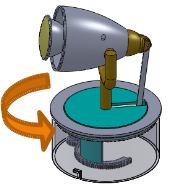
\includegraphics[scale=0.3]{./figures/spot3.png}
		\end{center}
	\end{minipage}
	\hfill
	\begin{minipage}[b]{0.48\linewidth}
		\scriptsize
		\begin{itemize}
			\item Traduction en exigence
		\end{itemize}
		\begin{center}
			\vspace{-1em}
		\begin{tikzpicture}[scale=0.6]
			\node[draw,rectangle,align=center,minimum width=4cm, fill=lred] (title) at (0,0) {\og{}requirement\fg{} \\ \textbf{Réglage de l'orientation}};
			\node[draw,rectangle,align=left,minimum width=4cm] (title) at (0,-1.8) {Id=\og{}003\fg{} \\ Text= \og{}On doit pouvoir \\ facilement orienter le spot\fg{}};
		\end{tikzpicture}
		\end{center}
	\end{minipage}
}

\frame{
	\frametitle{req : exemple du spot lumineux}
	\begin{minipage}[b]{0.65\linewidth}
		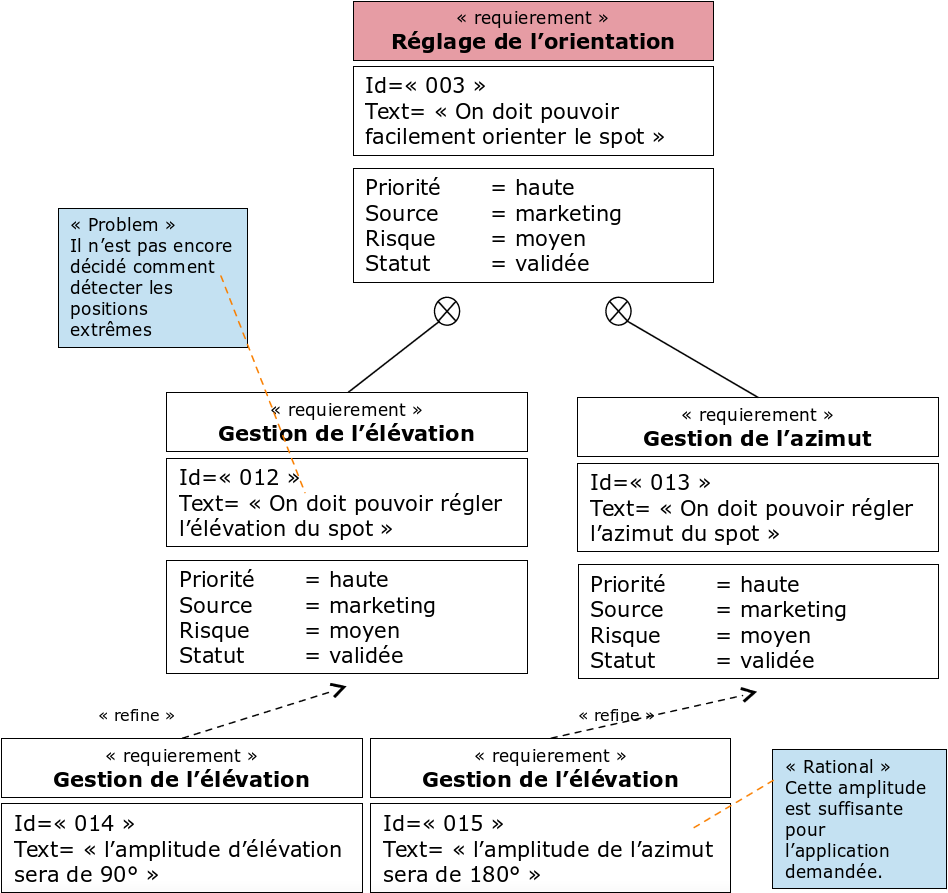
\includegraphics[width=\linewidth]{./figures/req1.png}
	\end{minipage}
	\hfill
	\begin{minipage}[b]{0.34\linewidth}
		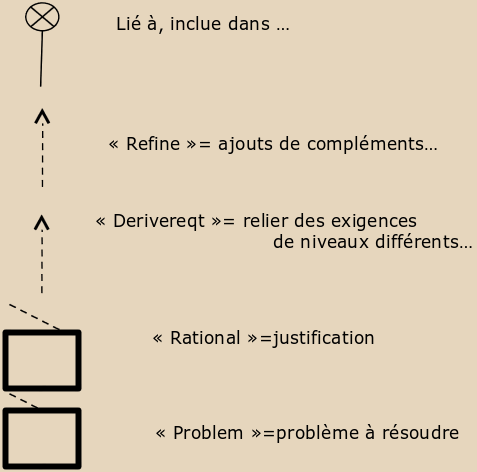
\includegraphics[width=\linewidth]{./figures/req2.png}
		\vspace{3cm}
	\end{minipage}
}

\section[bdd]{Diagramme de définition de block}
\subsection[bdd]{Diagramme de définition de block}
\frame{
	\frametitle{Diagramme d'exigences}
	\begin{center}
		\tiny
		\begin{tikzpicture}[scale=.6]
			\draw[drop shadow, fill=lorange] (-2.5,-0.5) rectangle (2.5,0.5);
			\draw (0,0) node{Diagramme SysML};

			\draw[drop shadow, fill=lorange] (-7.5,-1.5) rectangle (-2.5,-2.5);
			\draw (-5,-2) node{Diagramme comportemental};

			\draw[drop shadow, fill=lorange] (7.5,-1.5) rectangle (2.5,-2.5);
			\draw (5,-2) node{Diagramme structurel};

			\draw[drop shadow, fill=lyellow] (-1.5,-1.5) rectangle (1.5,-2.5);
			\draw (0,-2) node[align=center]{Diagramme \\ d'exigences};

			\draw[drop shadow, fill=gray] (-9.5,-3.5) rectangle (-6.5,-4.5);
			\draw (-8,-4) node[align=center]{Diagramme \\ d'activité};

			\draw[drop shadow, fill=lyellow] (-5.5,-3.5) rectangle (-2.5,-4.5);
			\draw (-4,-4) node[align=center]{Diagramme \\ d'états};

			\draw[drop shadow, fill=lyellow] (-0.5,-3.5) rectangle (2.5,-4.5);
			\draw (1,-4) node[align=center]{Diagramme de \\ définition de block};

			\draw[drop shadow, fill=lyellow] (3.5,-3.5) rectangle (6.5,-4.5);
			\draw (5,-4) node[align=center]{Diagramme de \\ bloc interne};

			\draw[drop shadow, fill=gray] (7.5,-3.5) rectangle (10.5,-4.5);
			\draw (9,-4) node[align=center]{Diagramme de \\ packages};

			\draw[drop shadow, fill=lyellow] (-8.5,-5.5) rectangle (-5.5,-6.5);
			\draw (-7,-6) node[align=center]{Diagramme de \\ séquence};

			\draw[drop shadow, fill=lyellow] (-5,-5.5) rectangle (-1,-6.5);
			\draw (-3,-6) node[align=center]{Diagramme de cas \\ d'utilisation};

			\draw[drop shadow, fill=gray] (3.5,-5.5) rectangle (6.5,-6.5);
			\draw (5,-6) node[align=center]{Diagramme \\ paramétrique};

			\draw (-5,-1.5) -- (-5,-1) -- (5,-1) -- (5,-1.5);
			\draw[->] (0,-1.5) -- (0,-0.5);

			\draw (-8,-3) -- (-2,-3);
			\draw (-8,-3.5) -- (-8,-3);
			\draw (-4,-3.5) -- (-4,-3);
			\draw (-6,-5.5) -- (-6,-3);
			\draw (-2,-5.5) -- (-2,-3);
			\draw[->] (-5,-3) -- (-5,-2.5);

			\draw (1,-3.5) -- (1,-3) -- (9,-3) -- (9,-3.5);
			\draw[->] (5,-3.5) -- (5,-2.5);
			
			\draw[->] (5,-5.5) -- (5,-4.5);

			\draw[ultra thick, gray, rounded corners=3] (-5.2,-5.3) rectangle (-0.8,-6.7);
			\draw[ultra thick, gray, rounded corners=3] (-1.7,-1.3) rectangle (1.7,-2.7);
			\draw[ultra thick, red, rounded corners=3] (-0.7,-3.3) rectangle (2.7,-4.7);
		\end{tikzpicture}
	\end{center}
}

\frame{
	\frametitle{Diagramme de définition de block}
	\begin{center}
		\small
		\textbf{En anglais :} \emph{Block definition diagram}\\
		\textbf{Abrégé :} \texttt{bdd}
		\footnotesize
		\begin{block}{Définition}
			Le \textbf{diagramme de définition de blocs} est similaire à la première page d’une notice de montage, 
			indiquant la liste des éléments et des pièces à assembler.
		\end{block}
		\begin{block}{}
			Ainsi le \textbf{bloc principal} et la \textbf{hiérarchie des blocs} qui le composent, qu’ils soient logiciels ou matériels, sont spécifiés dans ce diagramme.
		\end{block}
	\end{center}

}

\section[s2]{S2}
\subsection[su1]{SU1}
\frame{
	\frametitle{Contexte}
	\center
	blbl
}
\subsection[su2]{SU2}
\frame{
	\frametitle{Contexte}
	\center
	blbl
}

\end{document}


